\chapter{Appendix}

\section{Calculations}



Calculate creation and annihilation operator in k-space (symmetric normation factors):
\begin{align}
c_{2n} &= \frac{1}{\sqrt{N_d}}\sum_k\exp\left[ik\left(2n\right)a\right]\cdot c_{k}^{(e)}\\
c_{2n+1} &= \frac{1}{\sqrt{N_d}}\sum_k\exp\left[ik\left(2n+1\right)a\right]\cdot c_{k}^{(o)}\\
c_k^{(e)} &= \frac{1}{\sqrt{N_d}}\sum_n \exp\left[-ik\left(2n\right)a\right]\cdot c_{2n}\\
c_k^{(o)} &= \frac{1}{\sqrt{N_d}}\sum_n \exp\left[-ik\left(2n+1\right)a\right]\cdot c_{2n+1}
\end{align}
Remember: operators $c_{2n(+1)}$ operate on double unit cell length $\rightarrow$ halve Brillouin zone $\left(-\frac{\pi}{2a}, \frac{\pi}{2a}\right]$\\
boundary condition: $\exp\left[2ik\left(n+N_d\right)a\right] = 1 \rightarrow N_d$ allowed kpts in Brillouin zone\\
Check for $c_{2n}$:
\begin{align}
c_{2n_0}(c_k^{(e)}(c_{2n_i})) &= c_{2n} \\
&= \frac{1}{\sqrt{N_d}}\sum_k\exp\left[ik\left(2n_0\right)a\right]\cdot \frac{1}{\sqrt{N_d}}\sum_n \exp\left[-ik\left(2n\right)a\right]\cdot c_{2n}\\
&= \frac{1}{N_d}\sum_{k, n} \exp\left[ika\left(2n_0-2n\right)\right]\cdot c_{2n}\\
&= \frac{1}{N_d}\sum_n N_d \delta_{2n_0,2n} c_{2n}\\
&= c_{2n_0}
\end{align}
Warm up calculation:
\begin{align}
\sum_n^{N_d}c_{2n+1}^\dagger c_{2n} &=\sum_{n, k, k'} \exp\left[ika(2n)\right] \cdot \exp\left[-ik'a(2n+1)\right] \cdot \frac{c_{k'}^{\dagger(o)}c_k^{(e)}}{N_d} \\
&=\sum_{n, k, k'} \exp\left[ia(k-k')(2n)\right] \cdot \exp\left(-ik'a\right) \cdot  \frac{c_{k'}^{\dagger(o)}c_k^{(e)}}{N_d} \\
&=\sum_{k, k'} \delta_{k, k'} \cdot \exp\left(-ik'a\right)\cdot c_{k'}^{\dagger(o)}c_k^{(e)}\\
&=\sum_{k'} \exp\left(-ik'a\right) \cdot c_{k'}^{\dagger(o)}c_{k'}^{(e)}
\end{align}
Analogously:
\begin{align}
\sum_n^{N_d} c_{2n}^\dagger c_{2n+1} &=\sum_{k'} \exp\left(ik'a\right)\cdot c_{k'}^{\dagger(e)}c_{k'}^{(o)}\\
\sum_n^{N_d} c_{2n}^\dagger c_{2n-1}&=\sum_{k'} \exp\left(-ik'a\right)\cdot  c_{k'}^{\dagger(e)}c_{k'}^{(o)}\\
\sum_n^{N_d} c_{2n-1}^\dagger c_{2n} &=\sum_{k'} \exp\left(ik'a\right)\cdot  c_{k'}^{\dagger(o)}c_{k'}^{(e)}
\end{align}
Thus one obtains:
\begin{align}
\mathcal{H} &= -2\sum_n^{N_d} \left[\left(t_0+\delta\right)\left(c_{2n+1}^\dagger c_{2n} + c_{2n}^\dagger c_{2n+1} \right) + 
\left(t_0-\delta\right)\left(c_{2n+2}^\dagger c_{2n+1} + c_{2n+1}^\dagger c_{2n+2}\right)\right]+2N\kappa u^2\\
&= -2\sum_{k'} \left[\left(t_0+\delta\right)\left(\exp\left(-ik'a\right) \cdot c_{k'}^{\dagger(o)}c_{k'}^{(e)} + \exp\left(ik'a\right)\cdot c_{k'}^{\dagger(e)}c_{k'}^{(o)}\right)+ \right.\nonumber\\
&\hspace*{1.6cm}\left.\left(t_0-\delta\right)\left(\exp\left(-ik'a\right)\cdot  c_{k'}^{\dagger(e)}c_{k'}^{(o)}+\exp\left(ik'a\right)\cdot  c_{k'}^{\dagger(o)}c_{k'}^{(e)}\right)\right]+2N\kappa u^2\\
&= -2\sum_{k'} \left\{\left[2t_0\cos(k'a) + 2i\delta\sin(k'a)\right]c_{k'}^{\dagger(e)}c_{k'}^{(o)} + \right.\nonumber\\
&\hspace*{1.7cm}\left. \left[2t_0\cos(k'a)-2i\delta\sin(k'a)\right] c_{k'}^{\dagger(o)}c_{k'}^{(e)}\right\}+2N\kappa u^2\\
&\neq-2\sum_{k'} \left\{\left[\textcolor{red}{-}2t_0\cos(k'a) + 2i\delta\sin(k'a)\right]c_{k'}^{\dagger(e)}c_{k'}^{(o)} + \right.\nonumber\\
&\hspace*{1.7cm}\left. \left[\textcolor{red}{-}2t_0\cos(k'a)-2i\delta\sin(k'a)\right] c_{k'}^{\dagger(o)}c_{k'}^{(e)}\right\}+2N\kappa u^2
\end{align}
Substituting $\epsilon_k := 2t_0\cos(ka)$ and $\Delta_k := 2\delta\sin(ka)$ the following form of the hopping term can be derived:
\begin{align}
\mathcal{H}_{\text{hopp},k} &=
\left[\epsilon_k + i\Delta_k\right]c_{k}^{\dagger(e)}c_{k}^{(o)} + \left[\epsilon_k-i\Delta_k \right]	c_{k}^{\dagger(o)}c_{k}^{(e)}
\end{align}

Using this the ground state energy can be derived as follows (completely occupied valence, empty conduction band):
\begin{align}
E_0(u) &=-2\sum_k |E_k|\\
&= -2\sum_k \sqrt{\epsilon_k^2+\Delta_k^2}\\
&= -2\sum_k \sqrt{\left[2t_0\cos(ka)\right]^2+\left[2\delta\sin(ka)\right]^2}\\
\end{align}
In the limit of $N \rightarrow \infty$ the sum becomes an integral:
\begin{align}
E_0(u) &= \frac{-N}{\pi}\int\limits_{\nicefrac{-\pi}{2a}}^{\nicefrac{\pi}{2a}}\hspace*{-0.2cm}\text{d}k\ \sqrt{\left[2t_0\cos(ka)\right]^2+\left[2\delta\sin(ka)\right]^2} + 2N\kappa u^2\\
&=\frac{-4Nt_0}{\pi}\underbrace{\int\limits_{0}^{\nicefrac{\pi}{2}}\text{d}\theta\ \sqrt{1-\left(1-\frac{\delta^2}{t_0^2}\right)\sin^2(\theta)}}_{=:F(\nicefrac{\delta}{t_0})} + 2N\kappa u^2
\end{align}
For small $\nicefrac{\delta}{t_0}$ the integral can be approximated as follows:
\begin{align}
F\left(\frac{\delta}{t_0}\right) &\approx 1 + \frac{1}{2} \left[\ln\left(\frac{4|t_0|}{|\delta|}\right)-\frac{1}{2}\right]\frac{\delta^2}{t_0^2} 
\end{align}


To calculate the energies in manually charged states (cdft), use the states:
\begin{align}
\Psi_k^{(v)}(q) &= \sqrt{\frac{1}{2}-\frac{q}{2}}c_k^{\dagger(e)}- \sqrt{\frac{1}{2}+\frac{q}{2}}\frac{\epsilon_k - i \Delta_k}{|E_k|}c_{k}^{\dagger(o)}
\end{align}
To test for the correct properties one calculates $\left|\left\langle c^{(*)}_k|\Psi_k^{(v)}(q)\right\rangle\right|^2$, for example:
\begin{align}
\left|\left\langle c^{\dagger(e)}_k|\Psi_k^{(v)}(q)\right\rangle\right|^2 &= \left|c_k^{(e)} \left(\sqrt{\frac{1}{2}-\frac{q}{2}}c_k^{\dagger(e)}- \sqrt{\frac{1}{2}+\frac{q}{2}}\frac{\epsilon_k - i \Delta_k}{|E_k|}c_{k}^{\dagger(o)}\right)\right|^2\\
&= \frac{1-q}{2}
\end{align}
Because of the two different spin orientations of the electron an additional factor 2 has to be taken into account to get the correct number of valence electrons at the even/odd positions. Therefore the number of valence electrons is given by $1 \pm q$. The energies for this states are given by:
\begin{align}
\left\langle\Psi_k^{(v)}(q)\Big|\mathcal{H}_{\text{hopp},k}\Big|\Psi_k^{(v)}(q)\right\rangle &= \left[\sqrt{\frac{1-q}{2}}c_k^{(e)}- \sqrt{\frac{1+q}{2}}\frac{\epsilon_k + i \Delta_k}{|E_k|}c_{k}^{(o)}\right]\cdot\nonumber\\
&\hspace*{0.5cm}\left[
\left[\epsilon_k + i\Delta_k\right]c_{k}^{\dagger(e)}c_{k}^{(o)} + \left[\epsilon_k-i\Delta_k \right]	c_{k}^{\dagger(o)}c_{k}^{(e)}
\right]\cdot\nonumber\\
&\hspace*{0.5cm}\left[\sqrt{\frac{1-q}{2}}c_k^{\dagger(e)}- \sqrt{\frac{1+q}{2}}\frac{\epsilon_k - i \Delta_k}{|E_k|}c_{k}^{\dagger(o)}\right]\\
&=-\sqrt{\frac{1-q}{2}}c_k^{(e)}\left[\epsilon_k+i\Delta_k \right]	c_{k}^{\dagger(e)}c_{k}^{(o)}\sqrt{\frac{1+q}{2}}\frac{\epsilon_k - i \Delta_k}{|E_k|}c_{k}^{\dagger(o)}\nonumber\\
&\hspace*{0.4cm}-\sqrt{\frac{1+q}{2}}\frac{\epsilon_k + i \Delta_k}{|E_k|}c_{k}^{(o)}\left[\epsilon_k - i\Delta_k\right]c_{k}^{\dagger(o)}c_{k}^{(e)}\sqrt{\frac{1-q}{2}}c_k^{\dagger(e)}\\
&=-\sqrt{\frac{1+q}{2}}\sqrt{\frac{1-q}{2}}\left[\frac{(\epsilon_k-i\Delta_k)(\epsilon_k+i\Delta_k)}{|E_k|}+\frac{(\epsilon_k-i\Delta_k)(\epsilon_k+i\Delta_k)}{|E_k|}\right]\\
&= -\sqrt{1-q^2} |E_k|
\end{align}
For this reason the expected ground state energy  as a function of the transferred charge in respect of a negligible small  phonon coupling constant $\delta$ has the form:
\begin{align}
E_0(q, u) &= -\frac{4Nt_0}{\pi} \sqrt{1-q^2} + 2N\kappa u^2
\end{align}  
Fit this function with simulation results for small q, see \cref{image_cdft_many_kpts}. Optimized fit coefficient:
\begin{align}
t_0 &= \unit[9,4]{eV}\qquad\text{from fit}\\
t_0 &= \unit[2.5]{eV}\qquad\text{Glen paper}
\end{align}
\begin{figure}
	\centering
	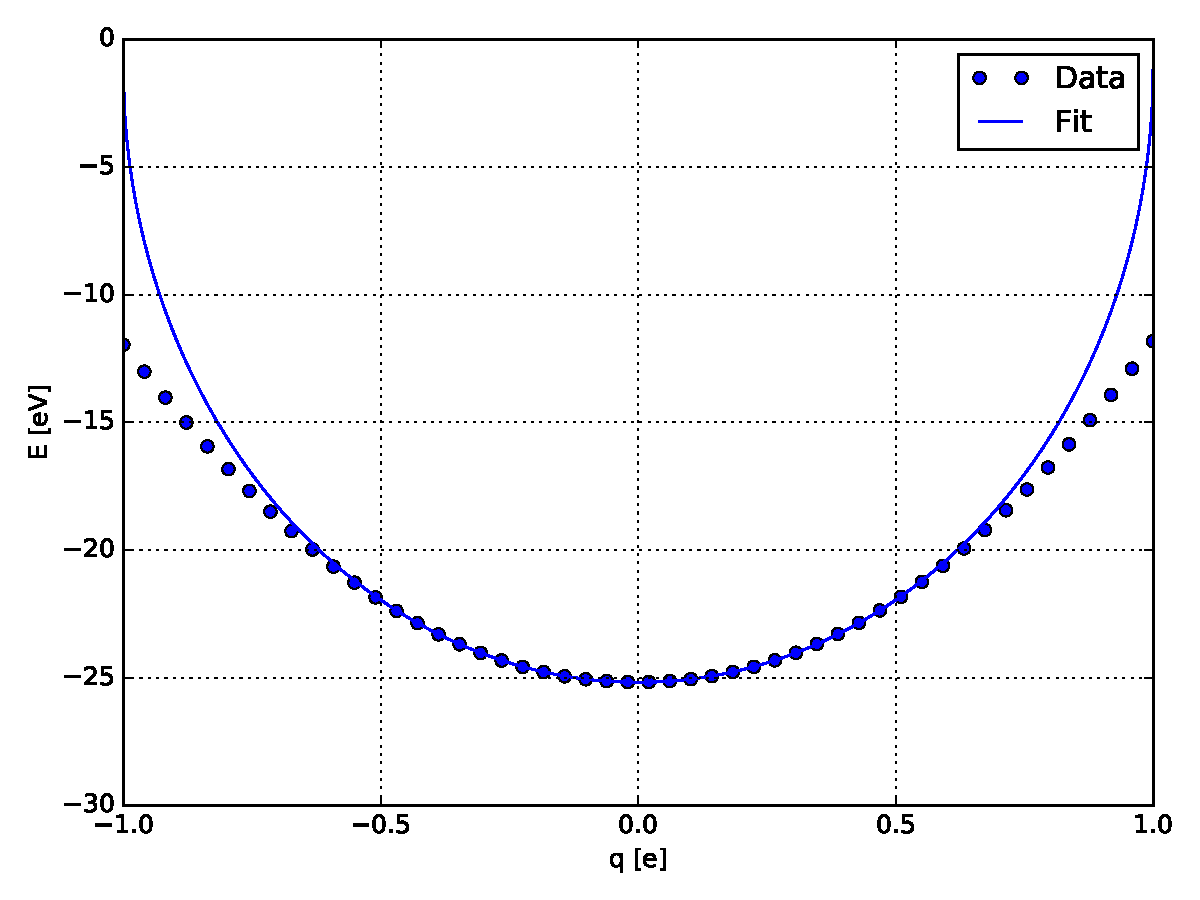
\includegraphics[width = \textwidth]{Images/CDFT/cdft_energy_many_kpts.pdf}
	\caption[Unit cell energy as function of the manually shiftet charge for many k-points]{Unit cell energy as function of the manually shiftet charge for many k-points}
	\label{image_cdft_many_kpts}
\end{figure}
Probably this assumption is wrong:
\begin{align}
\Psi_k^{(v)}(q) &= \sqrt{\frac{1-q}{2}}c_k^{\dagger(e)}- \sqrt{\frac{1+q}{2}}\frac{\epsilon_k - i \Delta_k}{|E_k|}c_{k}^{\dagger(o)}
\end{align}
and should rather be formulated in a more general way:
\begin{alignat}{3}
&&\Psi_k^{(v)}(q_k) &= \sqrt{\frac{1-q_k}{2}}c_k^{\dagger(e)}- \sqrt{\frac{1+q_k}{2}}\frac{\epsilon_k - i \Delta_k}{|E_k|}c_{k}^{\dagger(o)}\\
\Rightarrow&\qquad&\left\langle\Psi_k^{(v)}(q_k)\Big|\mathcal{H}_{\text{hopp},k}\Big|\Psi_k^{(v)}(q_k)\right\rangle &= -\sqrt{1-q^2_k} |E_k|
\end{alignat}
With this states one can easily calculate the number of valence electrons at the even/odd positions, for example :
\begin{align}
q_k &= \vv{\Psi}_k^{*\top}\cdot\begin{pmatrix*}[c]
1 & 0\\
0 & 0
\end{pmatrix*}\cdot \vv{\Psi}_k\\
&= \left[2\left(E_k^2\mp V|E_k|\right)\right]^{-1} \cdot \left(-V\pm |E_k|\right)^2\\
&= \frac{\left(-V \pm |E_k|\right)^2}{2\left(E_k^2\mp V|E_k|\right)}
\end{align}

Then the HOMO-band energy sum can be calculated as follows:
\begin{align}
E_0 &= -\sum_k |E_k|\\
&= -\sum_k \sqrt{V^2+\epsilon_k^2+\Delta_k^2}\\
&= -\sum_k \sqrt{V^2 + 4t_0^2\cos^2(ka) + 4 \delta^2\sin^2(ka)}\\
&= -\sqrt{V^2 + 4t_0^2}\sum_k \sqrt{1 - c^2 \cdot \sin^2(ka)}
\end{align} 
with $c^2 = \frac{4t_0^2-4\delta^2}{V^2+4t_0^2}$. In the limit of $N \to \infty$ (number of $k$-points is $\nicefrac{N}{2}$) the sum can be transformed into an integral:
\begin{align}
E_0 &= \frac{-N}{\pi} \sqrt{V^2+4t_0^2} \int\limits_{0}^{\nicefrac{\pi}{2}} \text{d}\theta \sqrt{1 - c^2 \cdot \sin^2(\theta)}\\
&= \frac{-N}{\pi} \sqrt{V^2+4t_0^2} \cdot F(\sqrt{1-c^2}) 
\end{align}
To write this expression as a function of the displaced charge a relationship between the potential $V$ and $q$ is needed:
\begin{align}
q &= \frac{2}{N} \sum_k q_k\\
&= \langle q_k\rangle\\
&= \left\langle\frac{\left(V + |E_k|\right)^2}{2\left(E_k^2+ V|E_k|\right)}\right\rangle\\
&= \frac{1}{2} \left(\left\langle\frac{E_k^2+VE_k}{E_k^2+VE_k}\right\rangle + V\left\langle\frac{1}{E_k}\right\rangle\right)\\
&= \frac{1}{2} \left(1 + V \left\langle\frac{1}{E_k}\right\rangle\right)
\end{align}